\section{Introduction}\label{sec:introduction}

From immersive communications, games, virtual production, to virtual try-on and virtual fitting rooms, having an accurate 3D presentation of the body of a person is fundamental. For this, one would typically need to use a professional 3D capture stage with many cameras pointing at the person in the center of the stage, and then put all the videos together using a 3D reconstruction algorithm, such as the ones proposed by \cite{guo2019relightables}, \cite{collet2015high} or \cite{pages2018affordable}. These setups are complex (huge amount of data to manage, complicated calibration processes, high processing times) and expensive (a high number of cameras, professional lighting, computers, GPUs, networks and more), so to overcome these challenges, modern deep learning techniques aim to simplify the capture process by replacing the multi-camera setup with a single camera, from a single viewpoint. For example, \cite{saito2019pifu}, \cite{saito2020pifuhd}, and \cite{xiu2022icon} generate a full body 3D model of a person, \cite{escribano2022texture} propose a way to generate the textures of occluded areas. However, all these techniques output relatively low-resolution considering the target application, and they struggle with complicated poses where depth is difficult to convey from a single viewpoint.

To overcome these challenges, some approaches include additional information into the capturing process, including depth, which typically comes from a consumer-level depth sensor. Although new generation consumer-level depth sensors have significantly improved during the last few years, they still present high levels of noise and sometimes fail to capture details when the subjects are at a distance where their body can be fully captured (at around 2m and farther), and they are still sensitive to sun light (which interferes with the infra-red light these sensors typically use), dark materials (which absorb infra-red light) and non-Lambertian surfaces. 

In this work, we propose a new approach to generate high-resolution depth maps of humans using a single low-resolution image as input, using denoising diffusion probabilistic models (DDPMs). Our multi-modal DDPM was trained using high-resolution depth maps, extracted from a large dataset of photorealistic 3D models captured by Volograms \citep{volograms2021}, which allows us to obtain depth maps with higher accuracy than consumer-level depth sensors.

% Featured Image
\begin{figure}[t]
  \centering
  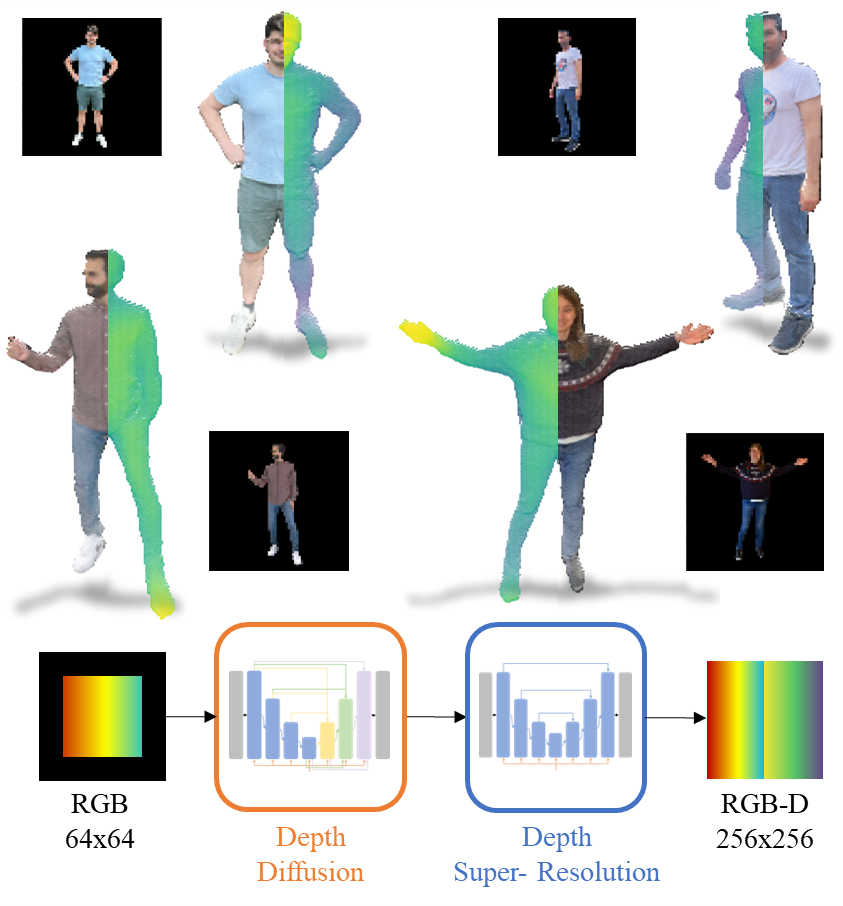
\includegraphics[width=0.99\linewidth]{illustrations/featured_image.png}
  \caption{Our \modelname{} framework generates a high-resolution RGB-D image from a low-resolution RGB image of humanoid subjects. First, a low resolution depth map is generated using a conditional DDPM. Then, the depth is upsampled to a higher resolution using a second DDPM.}
  \label{fig:featured_image}
\end{figure}

Following the taxonomy for multi-modal deep learning systems by \cite{zhan_multimodal_2022} we frame \modelname{} as a multi-modal generative translation task using a joint data representation of our input modalities RGB and depth. No alignment is performed between these modalities since our data is perfectly aligned during generation. We further perform parallel data co-learning since our RGB and depth pairs inherently share a direct correspondence between their instances.

We summarize our main contributions of this paper as follows:
\begin{enumerate}
  \item We provide a framework for high resolution dense monocular depth estimation using diffusion models.
  \item We perform super-resolution for dense depth data conditioned on a multi-modal RGB-D input condition using diffusion models. 
  \item We introduce a novel augmentation technique, namely depth noise, to enhance the robustness of the depth super-resolution model.
  \item We perform rigorous ablations and experiments to validate our design choices.
\end{enumerate}
